\section{Технологический раздел}
\subsection{Выбор языка и среды программирования}
В качестве языка программирования был выбран язык \texttt{C}. На этом языке реализованы все модули ядра и драйверы операционной системы \texttt{Linux}.

В качестве среды разработки был выбран текстовый редактор \texttt{Vim}.

\subsection{Структура ПО}

На рисунке \ref{fig:arch} представлена структура конечного ПО.

\begin{figure}[H]
	\centering
	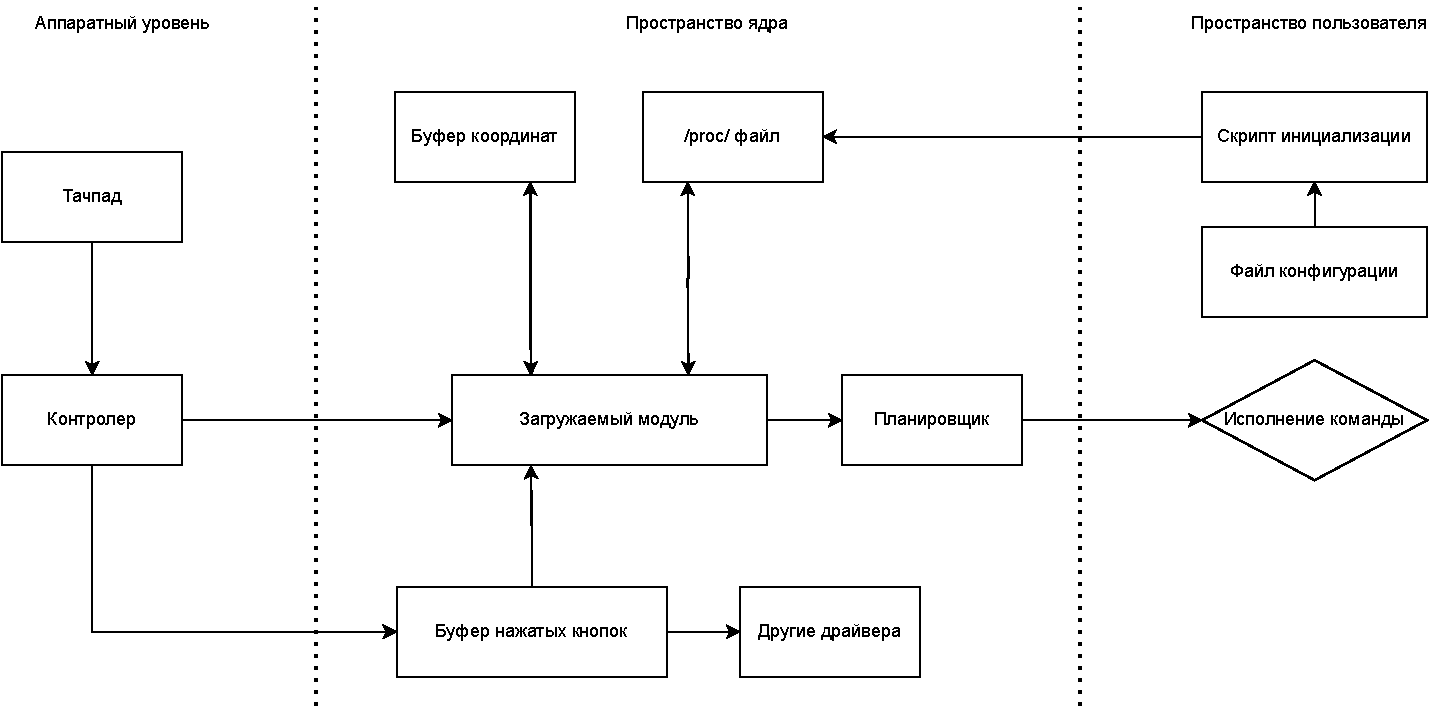
\includegraphics[width=0.9\textwidth]{inc/arch.pdf}
	\caption{Структура ПО}
	\label{fig:arch}
\end{figure}

\subsection{Функциональность разработанного ПО}

Одновременное касанием несколькими пальцами по тачпаду инициирует запись движения. После удаления пальцев с тачпада, записанное движение анализируется и сопоставляется с одним из шести шаблонов:
\begin{enumerate}
	\item вертикальное движение вверх;
	\item вертикальное движение вниз;
	\item горизонтальное движение (влево/вправо);
	\item движение в форме латинской буквы \texttt{V};
	\item движение по диагонали с правого верха, влево вниз;
	\item движение по диагонали с левого низа, вправо вверх.
\end{enumerate}

Функциональность тачпада сохраняется, ПО не влияет на действия с одним пальцем (перемещение курсора) и двумя пальцами (прокрутка).


\subsection{Инициализация структуры обработчика устройства ввода}

\begin{lstlisting}[label=lst:shandler,caption=Заполнение структур обработчика ввода, language=c]
	static const struct input_device_id touchpad_gest_ids[] = {
		{.driver_info = 1},
		{},
	};
	
	static struct input_handler touchpad_gest_handler = {
		.filter = touchpad_gest_filter,
		.connect = touchpad_gest_connect,
		.disconnect = touchpad_gest_disconnect,
		.name = DEVICE_NAME,
		.id_table = touchpad_gest_ids,
	};
\end{lstlisting}

Поля структуры:
\begin{itemize}
	\item filter -- обработчик событий;
	\item connect -- функция, вызываемая для подключении обработчика к устройству ввода;
	\item disconnect -- функция, вызываемая для отключения обработчика от устройства ввода;
	\item name -- имя обработчика (отображается в /proc/bus/input/handlers);
	\item id\_table -- указатель на таблицу идентификаторов устройств ввода, поддерживаемых драйвером.
\end{itemize}

\subsection{Инициализация структуры для создания файла в /proc/}

\begin{lstlisting}[label=lst:sproc,caption=Заполнение структуры proc, language=c]
	static struct proc_ops touchpad_gest_fops = {
		.proc_write = proc_write,
		.proc_read = proc_read};
\end{lstlisting}

Поля структуры:
\begin{itemize}
	\item proc\_write -- функция записи;
	\item proc\_read -- функция чтения;
\end{itemize}

\subsection{Листинг загружаемого модуля ядра}

Исходный код загружаемого модуля и файла сборки представлены в приложениях А и Б.

\clearpage